\section{Punto 1}
\textit{ Implementar el siguiente algoritmo de asignación de parejas}
\\
\underline{Problema:}

\textit{Pensar en una extensión del Problema de Asignaciones Estables de Gale and Shapley en la que ciertos pares hombre-mujer están explícitamente prohibidos.}\\

\textit{Dado un conjunto H de n hombres, un conjunto M de n mujeres y un conjunto de pares $P\subseteq H \times M$ que son aquellos que simplemente no están permitido emparejarse.}\\

\textit{Cada hombre h ranquea a todas las mujeres m tal que $(h, m) \notin P$, y cada mujer $m'$ ranquea a todos los hombres h' tal que $(h', m') \notin P$}

\textit{Entonces decimos que un macheo S es estable si no presenta ninguno de los siguientes tipos de inestabilidad:}

\begin{enumerate}[(i)]
  \item \textit{No existen dos pares $(h, m)$ y $(h', m')$ en S con la propiedad que si $(h, m') \notin P$, h prefiere a $m'$ en lugar de m, y $m'$ prefiere a h en lugar de h'. (Inestabilidad básica)}
  
  \item \textit{ Existe un par $(h, m) \in S$, y un hombre $h'$, tal que $h'$ no es parte de ningún par en el macheo, $(h', m) \in P$, y m prefiere a $h'$ en lugar de h. (Hombre soltero más deseable y no prohibido)}

  \item \textit{Existe un par $(h, m) \in S$, y una mujer $m'$, tal que $m'$ no es parte de ningún par en el macheo, $(h, m') \notin P$, y h prefiere a $m'$ en lugar de m. (Mujer soltera más deseable y no prohibida)}

  \item \textit{Existe un hombre h y una mujer m, ninguno de los cuales forman parte de una pareja en el emparejamiento, es decir $(h, m) \notin P$. (Hay dos personas solteras sin nada que les impida casarse entre ellas)}
\end{enumerate}

Se pide:

\begin{enumerate}[a)]
  \item \textit{Elegir las estructuras de datos adecuadas y justificar.}
  
  Para representar las preferencias de parejas se usaran matrices en donde los indices de las filas representaran al identificador de cada hombre/mujer, los indices de columnas representaran la prioridad en cuanto a preferencia, siendo el 0 la mayor preferencia, y los valores almacenados representaran a los identificador de cada mujer (que también serán representadas con indices pero de otra matriz). En la figura \ref{fig:MatricesPreferencia} se puede ver un ejemplo de las matrices de preferencia tanto de hombres como de mujeres.

  \begin{figure}[!htb]
    \centering
    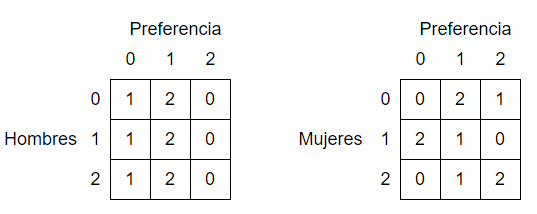
\includegraphics[width=\textwidth, scale=1]{Images/Punto1/MatricesPreferencia.png}
    \caption{Matrices de preferencia de hombres y mujeres}
    \label{fig:MatricesPreferencia}
  \end{figure}

  Para representar el conjunto de parejas que no están permitidos se utilizara una matriz donde los indices de las filas representaran a los hombres, los indices de las columnas a las mujeres y los valores almacenados serán 0 (Para indicar que una pareja con hombre de indice $i$ y mujer de indice $j$ no esta permitida) y 1 (Para indicar que una pareja con hombre de indice $i$ y mujer de indice $j$ esta permitida)

  Para finalizar se utilizaran dos arreglos, uno para las mujeres y otro para los hombres, donde se guardaran las parejas asignadas de cada uno, en donde los indices representaran a cada persona, es decir los indices del arreglo de hombres representaran a cada hombre y los indices del arreglo de mujeres representaran a cada mujer y el valor sera el indice representativo de la pareja de sexo opuesto asignada.
  
  En caso de que un hombre y mujer queden sin pareja a causa de las restricciones planteadas entonces sus valores en los arreglos de parejas tendrán el valor -1 para representar que justamente no se les pudo asignar una pareja.

  Los arreglos que se muestran en la figura \ref{fig:ArreglosParejas} representan el resultado del algoritmo sobre las matrices mostradas en las figuras \ref{fig:MatricesPreferencia} y \ref{fig:MatrizBan}, como se puede observar a causa de las restricciones planteadas el hombre 2 y la mujer 0 quedaron sin parejas asignadas.
  

  \begin{figure}[!htb]
    \centering
    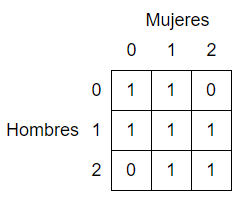
\includegraphics[width=8cm, scale=1]{Images/Punto1/No permitidas.png}
    \caption{Matriz de parejas no permitidas donde el hombre 0 y la mujer 2 es una pareja no permitida y el hombre 2 y la mujer 0 es otra pareja no permitida }
    \label{fig:MatrizBan}
  \end{figure}

  \begin{figure}[!htb]
    \centering
    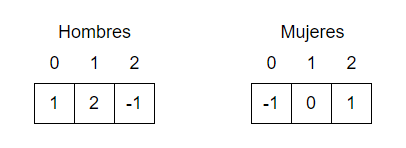
\includegraphics[width=15cm, scale=1]{Images/Punto1/Arreglos parejas.png}
    \caption{Arreglos de parejas asignadas}
    \label{fig:ArreglosParejas}
  \end{figure}
  \item \textit{Diseñar e Implementar en Java el algoritmo para resolver el problema}
  
  \begin{lstlisting}[style=java,caption= Implementacion problema de las parejas con asignaciones estables]
    public static void main(String[] args) {
      int[][] menPref = { //Indice fila es el hombre, indice col es la preferencia, valor es el indice mujer
              {1, 2, 0},
              {1, 2, 0}, 
              {1, 2, 0}, 
      };
      int[][] womenPref = { //Indice fila es el hombre, indice col es la preferencia, valor es el indice mujer
              {0, 2, 1}, 
              {2, 1, 0}, 
              {0, 1, 2},
      };
      int[][] bannedCouples = { //Indice fila es el hombre, indice col mujeres, 1 = pueden ser pareja, 0 = no pueden ser pareja
              {1, 1, 0},//Hombre 0 con mujer 2 no
              {1, 1, 1},
              {0, 1, 1}, //Hombre 2 con mujer 0 no
      };
      
      int[] womanCouples = new int[womenPref.length]; //indice hombres, -1 = sin pareja, otro valor indice de su pareja
      int[] manCouples = new int[menPref.length];
      assignCouples(menPref,womenPref,bannedCouples,manCouples,womanCouples);
  
      for (int i = 0; i < menPref.length; i++) {
        System.out.println("Hombre "+i+" --> "+" Mujer "+manCouples[i]);
      }
      for (int i = 0; i < womenPref.length; i++) {
        System.out.println("Mujer "+i+" --> "+" Hombre "+womanCouples[i]);
      }
    }
  
    public static int[] assignCouples(int[][] menPref, int[][] womenPref, int[][] bannedPartners, int[]manCouples,int[]womanCouples) {
      int amountMen = menPref.length;
      int freeMen = amountMen; //Cantidad de hombres restantes sin pareja
  
      Arrays.fill(manCouples, -1);//Inicialmente no tienen pareja
      Arrays.fill(womanCouples, -1);//Inicialmente no tienen pareja
      while (freeMen > 0) {//Mientras queden hombres sin pareja
        int indexMan = 0;
        while (indexMan < amountMen && manCouples[indexMan] > -1) {//Busca al siguiente hombre sin pareja
          indexMan++;
        }
        int indexPref = 0;
        while (indexMan < amountMen && manCouples[indexMan] == -1 && indexPref<womenPref.length) {
          int selectedWoman = menPref[indexMan][indexPref];
          if (bannedPartners[indexMan][selectedWoman] == 1) { //si pueden ser pareja
            if (womanCouples[selectedWoman] == -1) {//si mujer NO tiene pareja, los empajera
              womanCouples[selectedWoman] = indexMan;
              manCouples[indexMan] = selectedWoman; //Los empareja
              freeMen--; //Hay un hombre menos sin pareja
            } else {//Si la mujer tiene pareja
              int currentWomanCouple = womanCouples[selectedWoman];//Busca la pareja de la mujer
              if (betterCouple(womenPref, currentWomanCouple, indexMan)) {//Si el hombre actual es mejor pareja lo asigna
                womanCouples[selectedWoman] = indexMan;
                manCouples[currentWomanCouple] = -1; //La pareja actual deja de serlo
                manCouples[indexMan] = selectedWoman;//Se le asigna su nueva pareja
              }
            }
          }
          indexPref++;//Busca al siguiente hombre
        }
        //Si no encontro pareja es porque no se lo permitio la restriccion, por lo tanto quedara sin pareja
        //Para evitar bucle se decrementa en 1 la cantidad de hombres libres
        if(indexMan<amountMen && manCouples[indexMan]==-1){
          freeMen--;
        }
  
      }
      return womanCouples;
    }
  
  
    public static boolean betterCouple(int[][] womenPref,int currentWomanCouple, int newCouple){
      int indexCurrent = Arrays.asList(womenPref).indexOf(currentWomanCouple);
      int indexNew = Arrays.asList(womenPref).indexOf(currentWomanCouple);
      return indexNew < indexCurrent; //A menor indice mayor preferencia
    }
  \end{lstlisting}

  \item \textit{Calcular la eficiencia en tiempo y espacio.}
  
  Se deberá operar mientras queden hombres sin pareja por lo tanto se hará un recorrido equivalente a la cantidad de filas de la matriz de preferencias de hombres, luego se deberá ir recorriendo el arreglo de parejas de hombres buscando a los diferentes hombres que no tengan pareja, como este arreglo es igual a la cantidad de filas de la matriz de preferencia de los hombres entonces hasta el momento se tendrá $O(n^2)$.

  Finalmente se recorrerá la matriz de preferencia para cada hombre, es decir solamente su fila correspondiente que sera igual al numero de columnas del arreglo de preferencia, para buscar una mujer que se ajuste a sus preferencia por prioridad, luego internamente en esta repetitiva se aplica la lógica para ver si una mujer debe o no cambiar de pareja en función a sus preferencias pero al trabajar con indices no sera necesario recorrer su matriz de preferencia, si no que como cada hombre y mujer esta representado con indices se podrá acceder directamente al indice correspondiente que se desee checkear por lo que finalmente se tendrá un orden de ejecución $O(n\cdot m)$ en donde n sera el numero de hombres y m el numero de mujeres. Si se supone que se tiene la misma (o menos) cantidad de hombres que de mujeres se puede asegurar que se tiene un $O(n^2)$

  \item \textit{Demostrar la correctitud (termina, es correcto y es estable).}
  La correctitud se demostrara a partir de las siguientes reglas
  \begin{itemize}
    \item \textbf{Propiedad 1: }Los hombres se declaran a las mujeres en orden decreciente de preferencia siempre y cuando no conformen una pareja que no esta permitida
    \item \textbf{Propiedad 2: }Una vez que una mujer se empareja, solo cambia de estado para mejorar de pareja
  \end{itemize}

\textbf{Terminacion:}
  \begin{itemize}
    \item En cada iteración un hombre le propone salir a una mujer o como mínimo se lo propone, ya que para realizar la proposición primero debe verificarse que sea una pareja permitida
    \item Solo hay $n^2$ posibles comparaciones, suponiendo una misma cantidad de hombres que de mujeres
    \item Sea P(t) el conjunto de pares $(h, m)$ en los que $h$ le ha propuesto salir a una $m$ al final de la iteración t. Para todo $t$, P(t+1) es estrictamente mayor que P(t). Como solo hay $n^2$ posibles comparaciones, P(t) puede aumentar $n^2$ veces, entonces nunca habrá mas de $n^2$ iteraciones.
    Por lo tanto queda demostrada la terminación del algoritmo
  \end{itemize}

\textbf{Perfección (Demostración por reducción al absurdo): }
  \begin{itemize}
    \item Suponiendo que un hombre H no esta emparejado al terminar la ejecución del algoritmo
    \item Por lo anterior una mujer M no tendrá pareja
    \item Pero, por la propiedad 2, M no recibió ninguna proposición
    \item Sin embargo, H puede terminar sin pareja después de haberle propuesto (o haberse planteado hacerlo) salir a todas las mujeres
  \end{itemize}

  \textbf{Estabilidad (Demostración por reducción al absurdo): }Suponiendo que $(H,M)$ es una pareja inestable en el emparejamiento devuelto por el algoritmo
    \begin{enumerate}[1.]
      \item $H$ nunca le pidió salir a $M$ entonces $H$ prefiere a su pareja actual antes que a M o la propuesta generaría una pareja no permitida (propiedad 1) entonces $(H,M)$ es estable.
      \item $H$ le pidió salir a $M$ entonces $M$ rechazo a $H$ (directamente o después de encontrar a alguien mejor) entonces $M$ prefiere a su pareja actual antes que a H (propiedad 2) entonces $H,M$ es estable.
      \item En cualquier caso, $(H,M)$ es estable
    \end{enumerate}
  \item \textit{ Explicar de qué estrategia algorítmica se trata.}
  
  Se trata de una técnica de búsqueda local, es decir es que se puede tratar como un problema de optimización ya que se busca minimizar o maximizar algún valor (costo/beneficio), en este caso encontrar parejas con la mejor calidad posible en función a las preferencias, en este caso el método utilizado es mejora iterativa, este método lo que hace es comenzar con una posible solución que va mejorando a traves de aplicaciones repetidas de un paso simple. Funciona a partir de encontrar una primera solución relativamente fácil. Esta solución se podrá mejorar por una secuencia de cambios pequeños y finalizara cuando no se puedan hacer mas mejoras, por ejemplo las mujeres una vez que se les asigna una pareja luego pueden cambiarla por otra que se ajuste mas a sus preferencias
\end{enumerate}